\documentclass{urdpl}     % praca w języku polskim

% Lista wszystkich języków stanowiących języki pozycji bibliograficznych użytych w pracy.
% (Zgodnie z zasadami tworzenia bibliografii każda pozycja powinna zostać utworzona zgodnie z zasadami języka, w którym dana publikacja została napisana.)
\usepackage[english,polish]{babel}

% Użyj polskiego łamania wyrazów (zamiast domyślnego angielskiego).
\usepackage{polski}

\usepackage[utf8]{inputenc}

% dodatkowe pakiety
\usepackage{pdfpages}
\usepackage{mathtools}
\usepackage{amsfonts}
\usepackage{amsmath}
\usepackage{amsthm}
\usepackage[hidelinks]{hyperref}
\usepackage{float}
\usepackage{listings}
\usepackage{graphicx}
\usepackage{subcaption}
\usepackage{booktabs} % Dla \toprule, \midrule, \bottomrule
\usepackage{multirow} 
\usepackage{tabularx} 
\usepackage{amssymb} 
\usepackage{listings}
\usepackage{xcolor}
\usepackage{array}
\usepackage{makecell}
\usepackage[flushleft]{threeparttable}
\usepackage[normalem]{ulem}
\usepackage{lineno}

% --- < bibliografia > ---
\usepackage{csquotes}

% --- < listingi > ---

% Użyj czcionki kroju Courier.
\usepackage{courier}

\usepackage{listings}
\lstloadlanguages{TeX}
\renewcommand{\lstlistlistingname}{Spis listingów}
\renewcommand{\lstlistingname}{Listing}

\lstset{
	literate={ą}{{\k{a}}}1
           {ć}{{\'c}}1
           {ę}{{\k{e}}}1
           {ó}{{\'o}}1
           {ń}{{\'n}}1
           {ł}{{\l{}}}1
           {ś}{{\'s}}1
           {ź}{{\'z}}1
           {ż}{{\..z}}1
           {\u0104}{{\k{A}}}1
           {\u0106}{{\'C}}1
           {\u0118}{{\k{E}}}1
           {\u00d3}{{\'O}}1
           {\u0143}{{\'N}}1
           {\u0141}{{\L{}}}1
           {\u015a}{{\'S}}1
           {\u0179}{{\'Z}}1
           {\u017b}{{\..Z}}1,
	basicstyle=\footnotesize\ttfamily,
}

% styl dla kodu JAVA
\lstdefinestyle{javaStyle}{
    language=Java,
    basicstyle=\ttfamily\footnotesize,
    keywordstyle=\color{blue},
    commentstyle=\color{green!50!black}\itshape,
    stringstyle=\color{green},
    numberstyle=\tiny\color{gray},
    numbers=left,
    numbersep=5pt,
    stepnumber=1,
    showspaces=false,
    tabsize=2,
    showstringspaces=false,
    breaklines=true,
    breakatwhitespace=false,
    showtabs=false,
    keepspaces=true
}

\definecolor{stringcolor}{RGB}{163,21,21}
\definecolor{typecolor}{RGB}{43, 145, 176}

% --- < podpisy > ---
\AtBeginDocument{
	\renewcommand{\tablename}{Tabela}
	\renewcommand{\figurename}{Rys.}   
    \newcommand{\listingname}{Listing}
}

% --- < tabele > ---
\newcolumntype{C}[1]{>{\hsize=#1\hsize\centering\arraybackslash}X}

% --- < dane strony tytułowej > ---
\author{Yevhen Marchak}
\shortauthor{Y. Marchak}
\noAlbum{134945}

\titlePL{Aplikacja do zarządzania wizytami lekarskimi}
\titleEN{Medical Appointment Management Application}

\shorttitlePL{Aplikacja do zarządzania wizytami}
\shorttitleEN{Medical Appointment Management App}

\thesistype{Praca projektowa}

\thesisDone{Praca wykonana pod kierunkiem}
\supervisor{mgr inż. Ewa Żesławska}

\degreeprogramme{Informatyka}
\date{2025}

\department{Instytut Informatyki}
\faculty{Wydział Nauk Ściślych i Technicznych}

\setlength{\cftsecnumwidth}{10mm}
\setcounter{secnumdepth}{4}
\brokenpenalty=10000\relax

% --- < początek dokumentu > ---
\begin{document}

\titlepages

\fancypagestyle{plain}{
    \fancyhf{}
    \renewcommand{\headrulewidth}{0pt}
    \renewcommand{\footrulewidth}{0pt}
}

\setcounter{tocdepth}{2}
\tableofcontents
\clearpage

% --- < rozdziały > ---
\chapter*{Streszczenie}
\addcontentsline{toc}{chapter}{Streszczenie}

Celem niniejszego projektu było zaprojektowanie i zaimplementowanie aplikacji desktopowej do kompleksowego zarządzania wizytami lekarskimi. System umożliwia rejestrację i logowanie pacjentów oraz sekretariatu, przeglądanie i edycję danych pacjentów, lekarzy oraz historii wizyt. 

Zastosowano język Java 17, bibliotekę Swing do stworzenia graficznego interfejsu użytkownika oraz bazę danych PostgreSQL z obsługą poprzez JDBC. Projekt uwzględnia warstwową architekturę aplikacji, walidację danych oraz obsługę wyjątków.

Efektem pracy jest funkcjonalna i intuicyjna aplikacja wspomagająca zarządzanie procesem umawiania wizyt w placówce medycznej.

\vspace{1cm}

\chapter*{Abstract}
\addcontentsline{toc}{chapter}{Abstract}

The aim of this project was to design and implement a desktop application for comprehensive management of medical appointments. The system allows for registration and login of patients and secretaries, as well as browsing and editing data of patients, doctors, and visit history.

The project uses Java 17, the Swing library for GUI creation, and PostgreSQL with JDBC for database handling. It follows a layered architecture and includes data validation and exception handling.

The result is a functional and user-friendly application that supports the scheduling of appointments in a medical facility.
 
\chapter{Opis założeń projektu}

\section{Cel projektu}
Celem niniejszego projektu było stworzenie aplikacji desktopowej umożliwiającej kompleksowe zarządzanie wizytami lekarskimi. Aplikacja pozwala na przegląd, dodawanie, edycję oraz usuwanie informacji o pacjentach, lekarzach i wizytach.

\section{Zakres projektu}
Projekt obejmuje implementację:
\begin{itemize}
\item interfejsu graficznego w technologii \textbf{Swing},
\item komunikacji z relacyjną bazą danych PostgreSQL przez \textbf{JDBC},
\item systemu autoryzacji użytkowników (sekretariat, pacjent),
\item podstawowych operacji \textbf{CRUD} na danych,
\item walidacji, filtrowania, sortowania i obsługi wyjątków.
\end{itemize}

\section{Uzasadnienie wyboru tematu}
Temat został wybrany ze względu na jego praktyczne zastosowanie oraz popularność w instytucjach medycznych. Projekt umożliwił studentowi rozwój umiejętności z zakresu projektowania aplikacji wielowarstwowych, obsługi baz danych oraz projektowania GUI.

\section{Technologie}
W projekcie zastosowano:
\begin{itemize}
\item język programowania \textbf{Java 17},
\item bibliotekę \textbf{Swing} do interfejsu graficznego,
\item \textbf{PostgreSQL} jako system zarządzania bazą danych,
\item narzędzie \textbf{LaTeX} do przygotowania dokumentacji.
\end{itemize}

\section{Struktura pracy}
Praca składa się z sześciu głównych rozdziałów:
\begin{itemize}
\item Opis założeń projektu,
\item Opis struktury projektu,
\item Harmonogram realizacji projektu,
\item Prezentacja warstwy użytkowej projektu,
\item Implementacja projektu,
\item Testowanie i podsumowanie,
\end{itemize}

 
\chapter{Analiza i projekt systemu}

\section{Opis funkcjonalny systemu}
System zarządzania wizytami lekarskimi zapewnia funkcjonalność dla dwóch głównych typów użytkowników: \textbf{sekretariatu} oraz \textbf{pacjenta}. Każdy z użytkowników ma dostęp do dedykowanego panelu, zawierającego odpowiednie opcje i możliwości:

\begin{itemize}
  \item \textbf{Sekretariat:}
  \begin{itemize}
    \item przeglądanie, dodawanie, edytowanie i usuwanie danych pacjentów,
    \item zarządzanie wizytami: aktualizacja statusu, dodawanie notatek lekarskich,
    \item przeglądanie oraz zarządzanie lekarzami.
  \end{itemize}

  \item \textbf{Pacjent:}
  \begin{itemize}
    \item przeglądanie danych osobowych,
    \item przeglądanie historii wizyt wraz z notatkami od lekarza,
    \item rezerwacja nowej wizyty, wybierając lekarza i termin.
  \end{itemize}
\end{itemize}

\section{Diagram koncepcyjny bazy danych}
\begin{figure}[H]
\centering
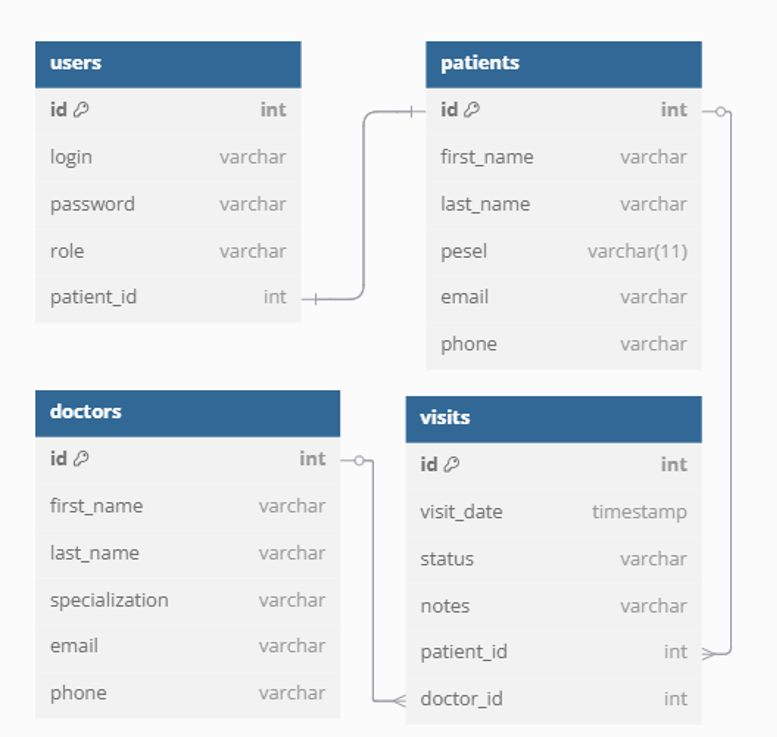
\includegraphics[width=0.85\textwidth]{figures/Diagram_bazy_danych.png}
\caption{Diagram koncepcyjny bazy danych}
\end{figure}

\section{Diagram klas (dziedziczenie)}
\begin{figure}[H]
\centering
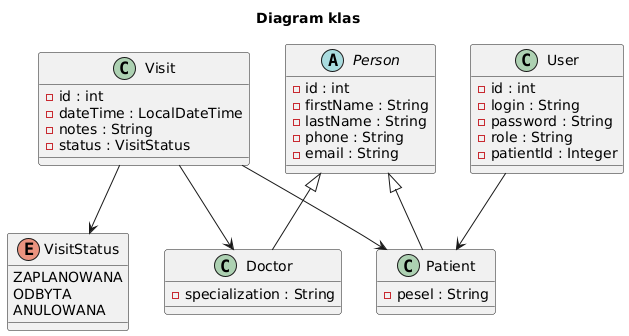
\includegraphics[width=0.85\textwidth]{figures/DiagramKlas.png}
\caption{Diagram klas przedstawiający hierarchię dziedziczenia}
\end{figure}

\section{Opis struktur danych}
System opiera się na czterech głównych encjach:
\begin{itemize}
  \item \textbf{Pacjent} -- dane identyfikacyjne (imię, nazwisko, PESEL, email, telefon),
  \item \textbf{Lekarz} -- imię, nazwisko, email, telefon, specjalizacja,
  \item \textbf{Wizyta} -- powiązanie lekarza z pacjentem, termin, status, notatka,
  \item \textbf{Użytkownik} -- login, hasło, rola (sekretarz lub pacjent), powiązanie z pacjentem (jeśli dotyczy).
\end{itemize}
 
\chapter{Harmonogram realizacji projektu}

\section{Etapy realizacji}

Prace nad projektem zostały podzielone na następujące etapy:

\begin{itemize}
  \item Zatwierdzenie tematu – 17.05.2025,
  \item Analiza i projekt systemu – 18.05–21.05.2025,
  \item Projekt bazy danych i diagram klas – 22.05–24.05.2025,
  \item Implementacja systemu (GUI, DAO, logika) – 25.05–02.06.2025,
  \item Obsługa wyjątków i walidacja – 03.06–05.06.2025,
  \item Testowanie aplikacji – 06.06–08.06.2025,
  \item Tworzenie dokumentacji – 09.06–14.06.2025,
  \item Ostateczne poprawki i złożenie – 15.06.2025.
\end{itemize}

\section{Wizualizacja harmonogramu}

Poniżej przedstawiono diagram Gantta obrazujący kolejne etapy realizacji projektu:

\begin{figure}[H]
\centering
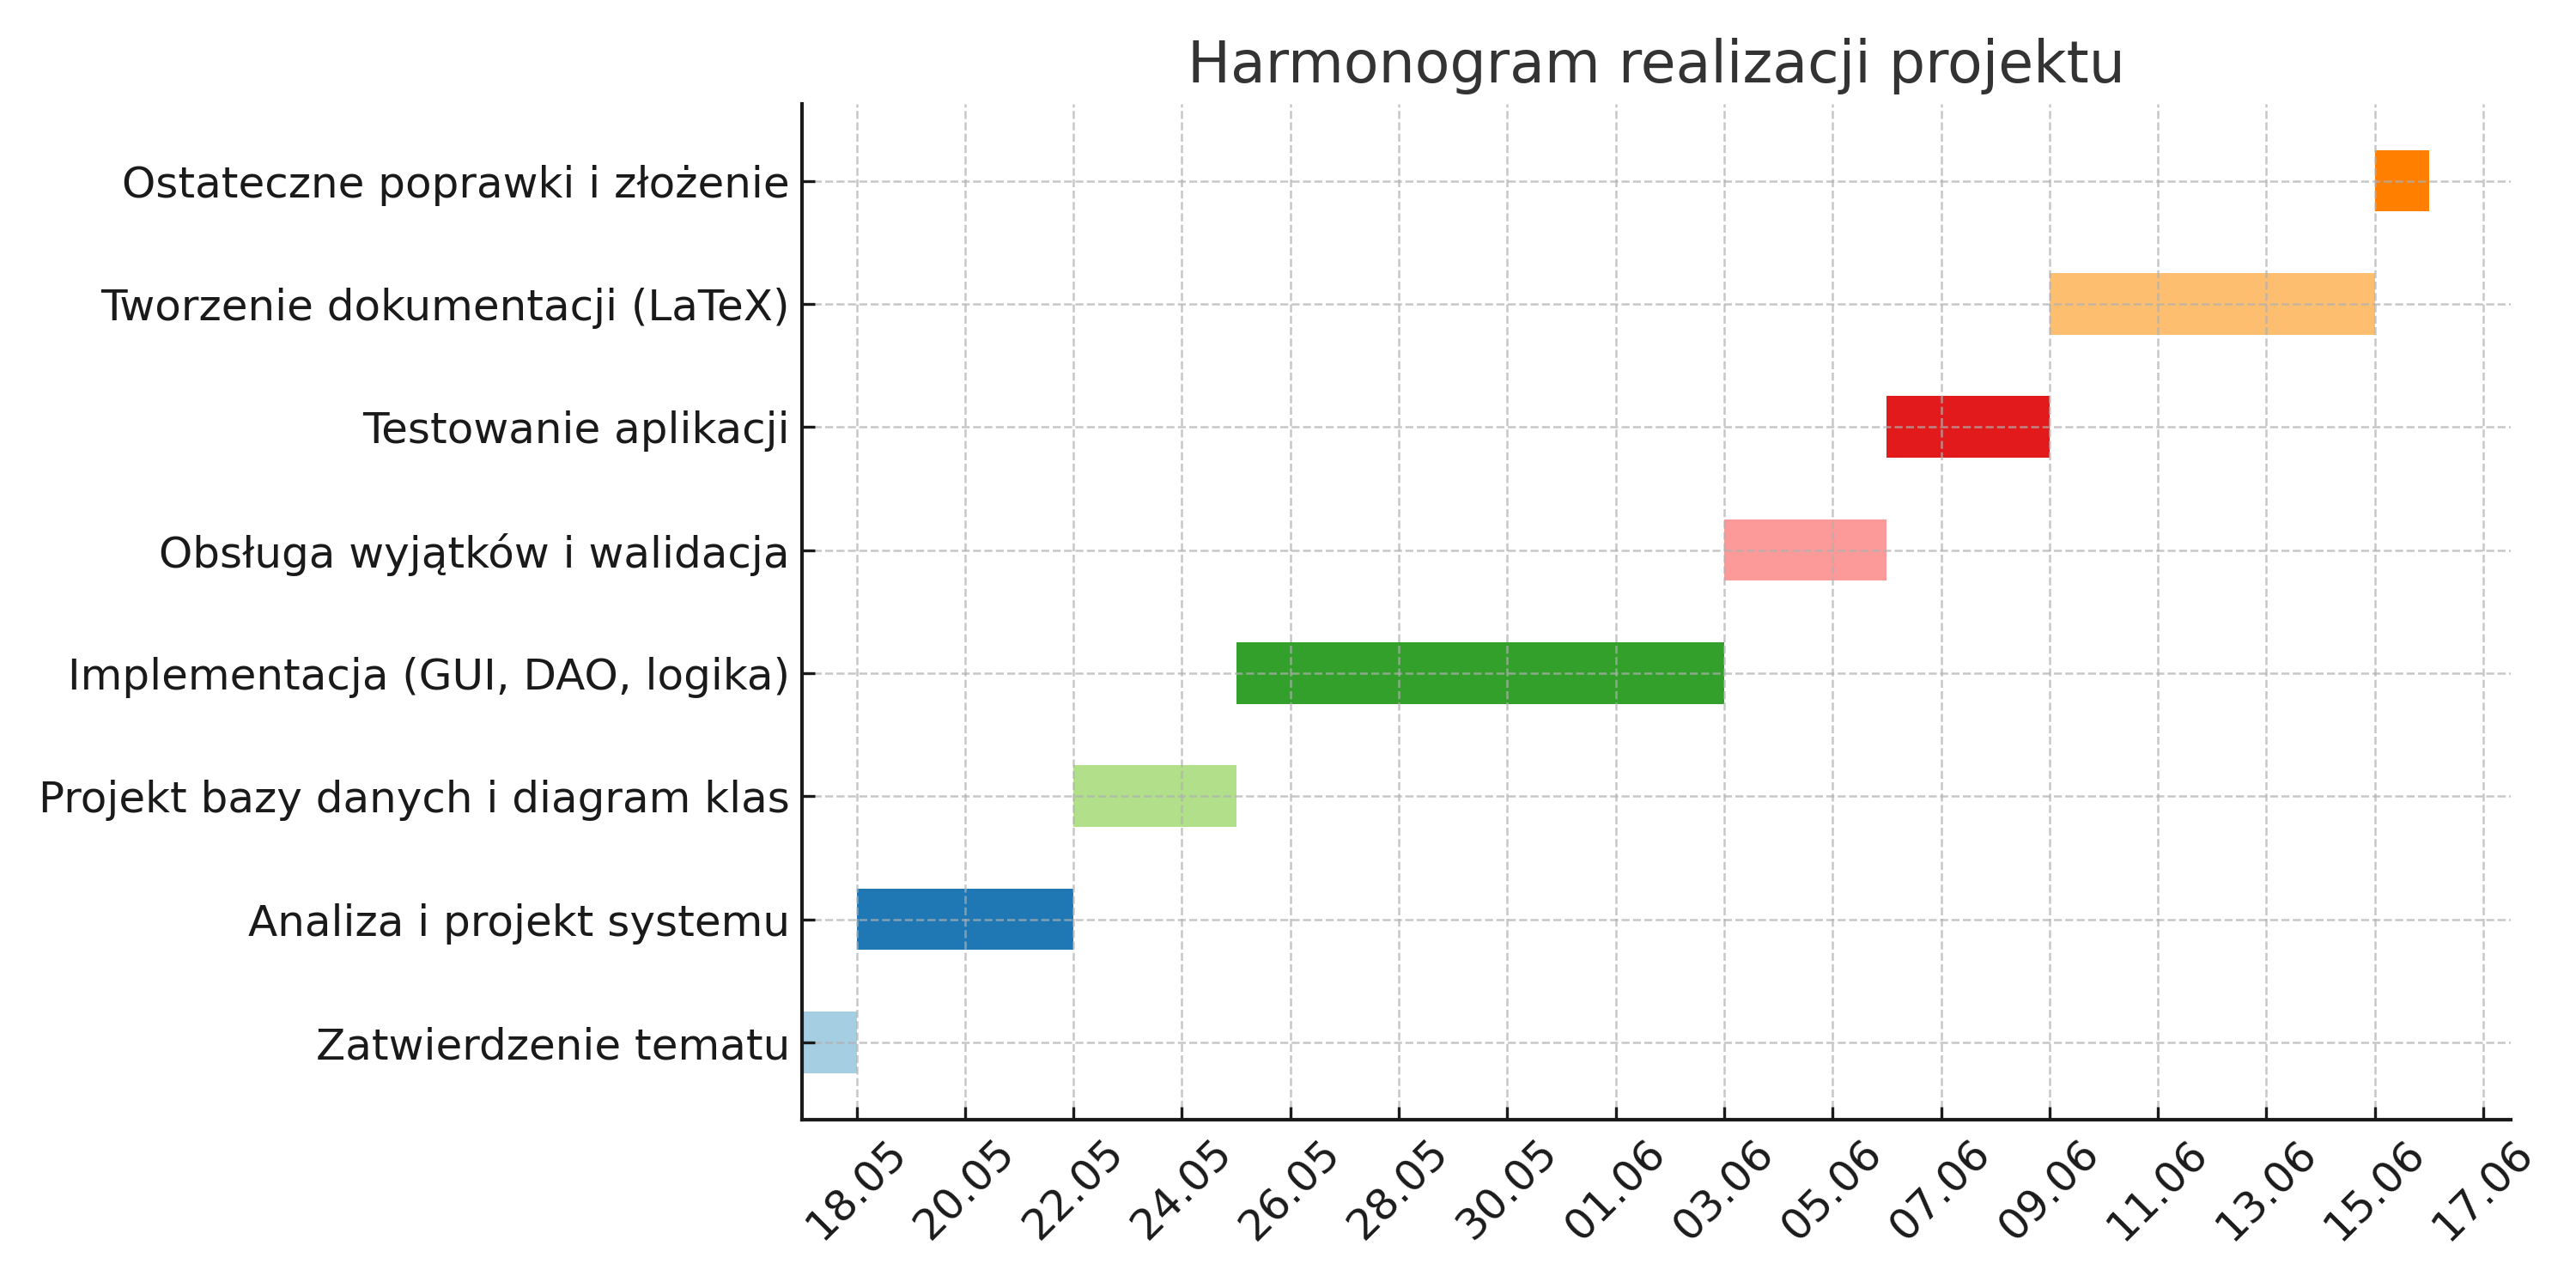
\includegraphics[width=0.95\textwidth]{figures/harmonogram_gantta.png}
\caption{Diagram Gantta – harmonogram realizacji projektu}
\end{figure}
 
\chapter{Prezentacja warstwy użytkowej projektu}

Graficzny interfejs użytkownika (GUI) został opracowany z myślą o prostocie obsługi, czytelności i intuicyjnej nawigacji. System udostępnia dwa główne panele: dla użytkownika typu \textbf{pacjent} oraz dla użytkownika typu \textbf{sekretariat}. Poniżej zaprezentowano poszczególne widoki oraz ich funkcjonalność.

\section{Okno powitalne}
To pierwsze okno aplikacji, z którego użytkownik może przejść do logowania lub zakończyć program.

\begin{figure}[H]
\centering
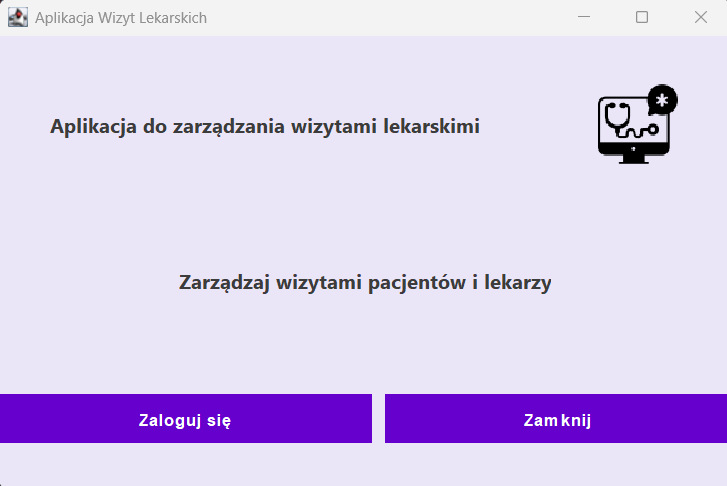
\includegraphics[width=0.7\textwidth]{figures/okno_powitalne.png}
\caption{Okno powitalne aplikacji}
\end{figure}

\section{Panel logowania}
Panel ten zawiera pola do wpisania loginu i hasła oraz przycisk do zalogowania. W przypadku błędnych danych użytkownik otrzymuje stosowny komunikat.

\begin{figure}[H]
\centering
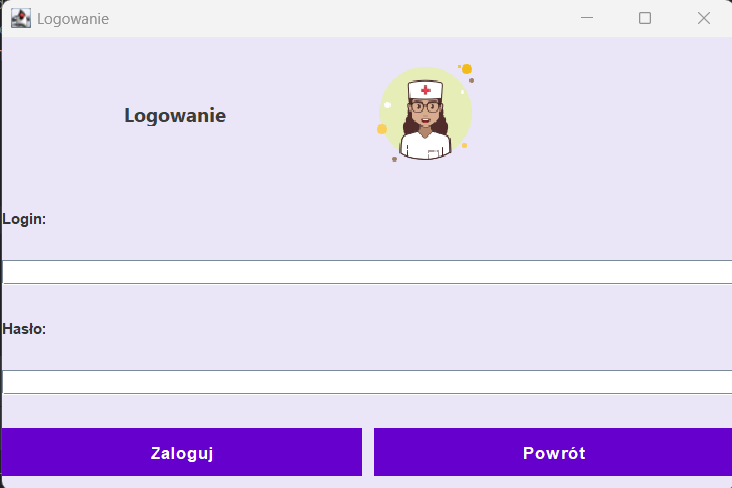
\includegraphics[width=0.7\textwidth]{figures/okno_logowania.png}
\caption{Ekran logowania}
\end{figure}

\section{Panel sekretariatu}
Po zalogowaniu się jako sekretarz użytkownik ma dostęp do głównego panelu zarządzania. Sekretariat może przeglądać, dodawać, edytować oraz usuwać dane pacjentów, lekarzy i wizyt.

\begin{figure}[H]
\centering
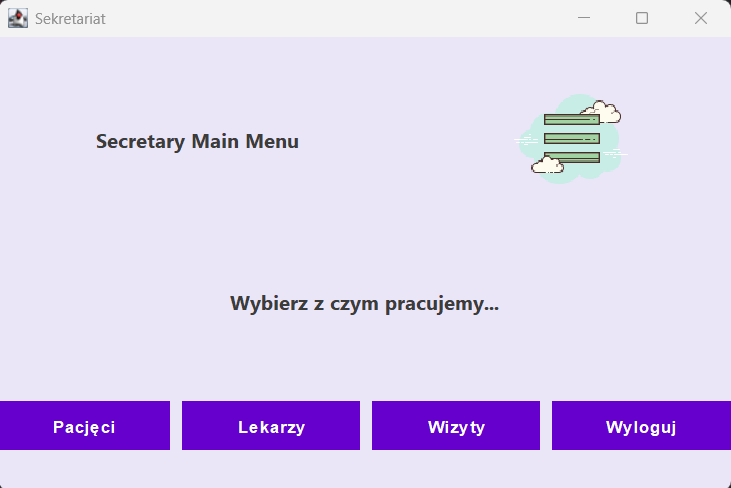
\includegraphics[width=0.75\textwidth]{figures/secretary_main_menu.png}
\caption{Główny panel sekretariatu}
\end{figure}

\section{Zarządzanie lekarzami}
Sekretariat posiada osobne okno do zarządzania lekarzami. W tym widoku możliwe jest przeglądanie listy wszystkich lekarzy oraz wykonywanie operacji CRUD (Dodaj, Edytuj, Usuń).

\begin{figure}[H]
\centering
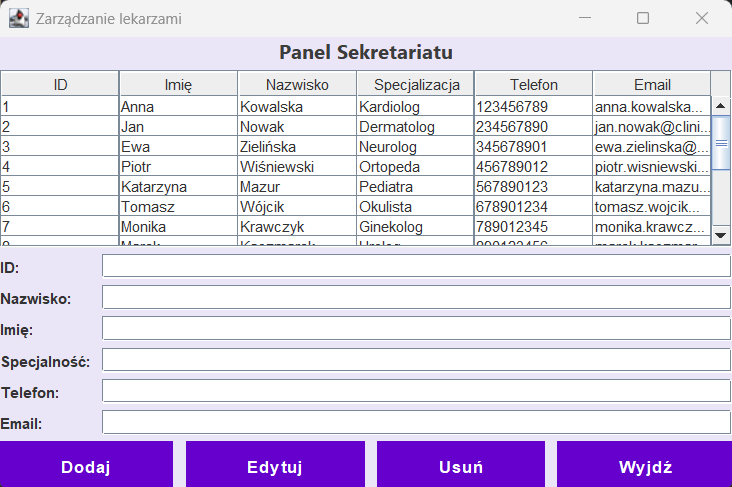
\includegraphics[width=0.75\textwidth]{figures/EditingDoctorsPanel.png}
\caption{Zarządzanie lekarzami – widok sekretariatu}
\end{figure}

\clearpage
\section{Panel pacjenta}
Po zalogowaniu się jako pacjent użytkownik ma dostęp do panelu z opcjami: „Moje dane”, „Moje wizyty”, „Zarezerwuj wizytę” oraz „Wyloguj”.

\begin{figure}[H]
\centering
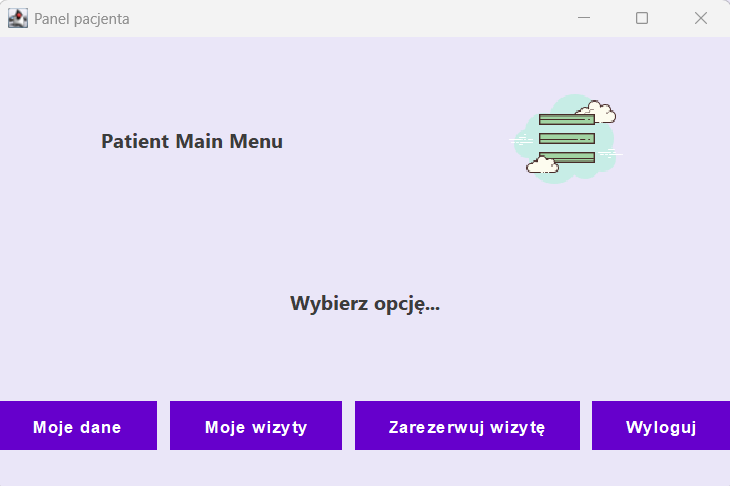
\includegraphics[width=0.75\textwidth]{figures/patient_panel.png}
\caption{Panel główny pacjenta}
\end{figure}


\section{Formularz danych pacjenta}
Panel „Moje dane” umożliwia pacjentowi podgląd danych osobowych, takich jak imię, nazwisko, PESEL, email oraz numer telefonu.

\begin{figure}[H]
\centering
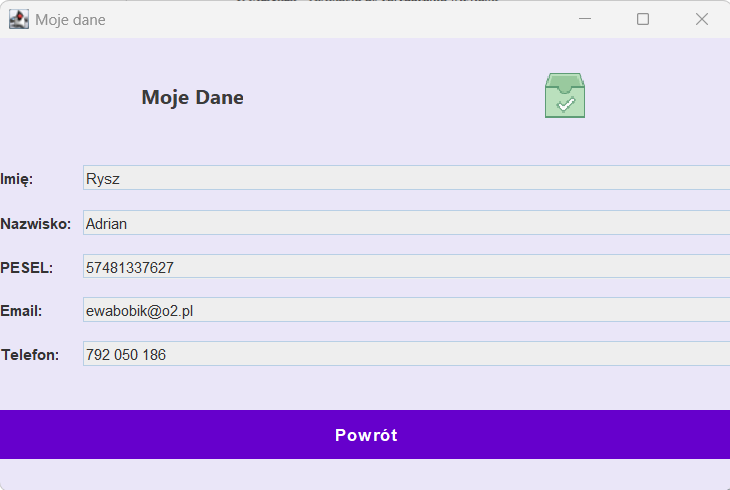
\includegraphics[width=0.7\textwidth]{figures/MyDataPatients.png}
\caption{Widok danych pacjenta}
\end{figure}
\clearpage
\section{Formularz rezerwacji wizyty}
W tym oknie pacjent może zarezerwować wizytę, wybierając lekarza z listy oraz wpisując dokładną datę i godzinę w formacie \texttt{YYYY-MM-DD HH:mm}.

\begin{figure}[H]
\centering
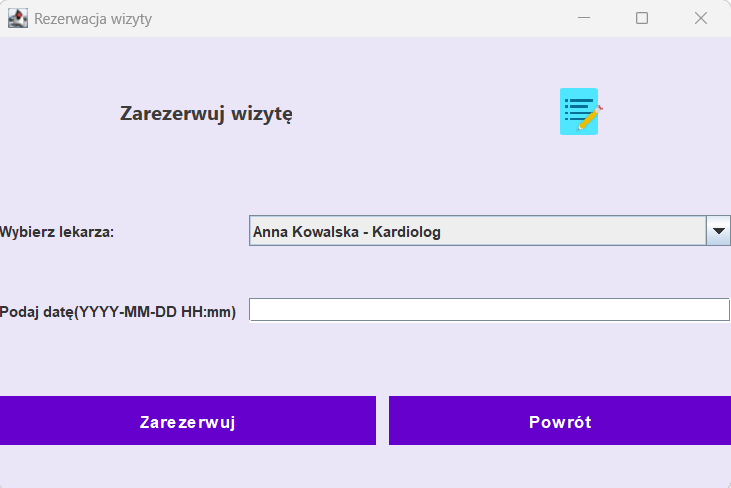
\includegraphics[width=0.7\textwidth]{figures/ReserveVisit.png}
\caption{Formularz rezerwacji wizyty}
\end{figure}

\section{Tabela wizyt}
Widok tabelaryczny wizyt umożliwia przeglądanie istniejących wpisów, filtrowanie oraz odświeżanie zawartości.

\begin{figure}[H]
\centering
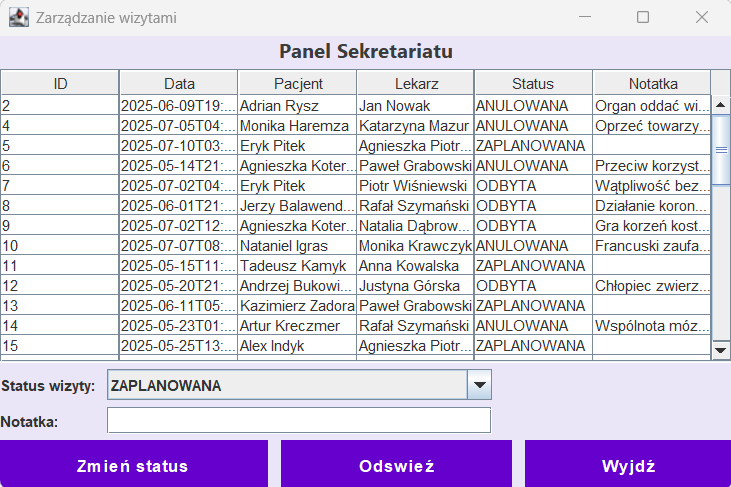
\includegraphics[width=0.7\textwidth]{figures/visit_table.png}
\caption{Tabela wizyt z funkcją odświeżania}
\end{figure}

\clearpage
\section{Tworzenie danych logowania pacjenta}
Podczas dodawania nowego pacjenta możliwe jest także automatyczne tworzenie konta użytkownika z przypisaną rolą.

\begin{figure}[H]
\centering
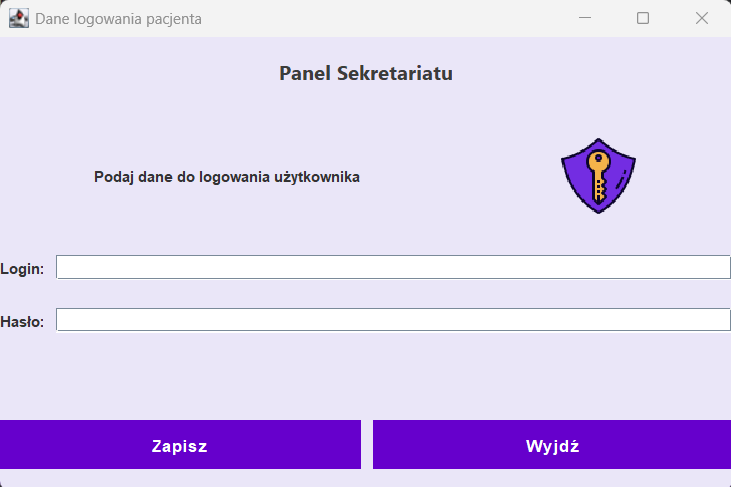
\includegraphics[width=0.7\textwidth]{figures/login_data.png}
\caption{Formularz do tworzenia konta pacjenta}
\end{figure}
 
\chapter{Implementacja}

W niniejszym rozdziale przedstawiono szczegóły implementacji systemu zarządzania wizytami lekarskimi, obejmujące strukturę projektu, zastosowane technologie oraz przykładowe fragmenty kodu źródłowego.

\section{Struktura projektu}

Projekt został zrealizowany zgodnie z podejściem warstwowym, obejmując następujące główne warstwy:

\begin{itemize}
\item \textbf{Warstwa danych} -- odpowiedzialna za komunikację z bazą danych PostgreSQL z wykorzystaniem JDBC,
\item \textbf{Warstwa logiki aplikacji} -- zarządzająca procesami biznesowymi, walidacją danych oraz obsługą wyjątków,
\item \textbf{Warstwa prezentacji} -- implementująca graficzny interfejs użytkownika (GUI) w technologii Swing.
\end{itemize}

\section{Technologie}

W projekcie wykorzystano następujące technologie:
\begin{itemize}
\item \textbf{Język Java 17} -- jako podstawowy język programowania,
\item \textbf{Swing} -- do stworzenia graficznego interfejsu użytkownika,
\item \textbf{PostgreSQL} -- jako system zarządzania bazą danych,
\item \textbf{JDBC} -- technologia do komunikacji z bazą danych,
\item \textbf{LaTeX} -- narzędzie do przygotowania dokumentacji.
\end{itemize}

\section{Kluczowe klasy}

Poniżej przedstawiono kluczowe klasy oraz ich role w systemie:

\begin{itemize}
\item \textbf{Doctor, Patient, Person} -- reprezentujące podstawowe jednostki w systemie,
\item \textbf{Visit} -- zarządzająca danymi dotyczącymi wizyt,
\item \textbf{User} -- obsługująca użytkowników systemu, ich logowanie oraz autoryzację,
\item \textbf{DoctorDAO, PatientDAO, VisitDAO} -- klasy zapewniające dostęp do danych z bazy.
\end{itemize}

\clearpage
\section{Przykładowe fragmenty kodu}

\subsection{Klasa Doctor}
\begin{lstlisting}[style=javaStyle,caption={Klasa reprezentująca lekarza — rozszerzenie klasy Person}]
public class Doctor extends Person {
        private String specialization;

        public Doctor(int id, String firstName, String lastName, String phone, String email, String specialization) {
            super(id, firstName, lastName, phone, email);
            this.specialization = specialization;
        }

        @Override
        public String getInfo() {
            return "Lekarz: " + firstName + " " + lastName + " - " + specialization;
        }

        public String getSpecialization() {
            return specialization;
        }

        public void setSpecialization(String specialization) {
            this.specialization = specialization;
        }

        @Override
        public String toString() {
            return firstName + " " + lastName + " - " + specialization;
        }

    }
\end{lstlisting}

\subsection{Metoda logowania użytkownika}
\begin{lstlisting}[style=javaStyle, caption={Metoda logowania użytkownika z wykorzystaniem JDBC}]
 public User login(String login, String password) {
        String sql = "SELECT * FROM users WHERE login = ? AND password = ?";

        try (Connection conn = DatabaseConnection.getConnection();
             PreparedStatement stmt = conn.prepareStatement(sql)) {

            stmt.setString(1, login);
            stmt.setString(2, password);

            try (ResultSet rs = stmt.executeQuery()) {
                if (rs.next()) {
                    return new User(
                            rs.getInt("id"),
                            rs.getString("login"),
                            rs.getString("password"),
                            rs.getString("role"),
                            rs.getObject("patient_id") != null ? rs.getInt("patient_id") : null
                    );
                }
            }

        } catch (SQLException e) {
            e.printStackTrace();
        }
        return null; //login lub hasło nie prawidłowe
    }
\end{lstlisting}

\section{Obsługa wyjątków i walidacja}
Aplikacja posiada zaimplementowaną obsługę wyjątków, mającą na celu zapewnienie stabilności oraz poprawności działania systemu. Poniżej przedstawiono przykładowe wyjątki wraz z fragmentami kodu oraz komunikatami wyświetlanymi użytkownikowi.

\subsection{Niepoprawne dane logowania}

W przypadku próby logowania przy użyciu błędnego loginu lub hasła wyświetlany jest odpowiedni komunikat błędu (Rys. \ref{fig:falseLogin}).

\begin{figure}[H]
\centering
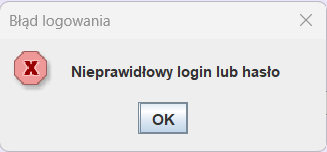
\includegraphics[width=0.5\textwidth]{figures/FalseDataforLogin.png}
\caption{Komunikat błędu - niepoprawne dane logowania}
\label{fig:falseLogin}
\end{figure}

Przykładowy fragment kodu:
\begin{lstlisting}[style=javaStyle, caption={Obsługa błędnego logowania — komunikat dla użytkownika}]
 if (user != null) {

    dispose();

        if (user.isSecretary()) {
            new SecretaryMainMenu().setVisible(true);
            } else if (user.isPatient()) {
                    PatientDAO patientDAO = new PatientDAO();
                    Patient patient = patientDAO.getPatientById(user.getPatientId());
                    if (patient != null) {
                    new PatientMainMenu(patient).setVisible(true);
                        } else {
                            JOptionPane.showMessageDialog(null, "Błąd: nie znaleziono danych pacjenta!", "Błąd", JOptionPane.ERROR_MESSAGE);
                        }
                    }
                }else {
                    JOptionPane.showMessageDialog(null, "Nieprawidłowy login lub hasło", "Błąd logowania", JOptionPane.ERROR_MESSAGE);
                }
\end{lstlisting}

\subsection{Istniejący login podczas rejestracji}

Przy próbie utworzenia nowego użytkownika z loginem, który już istnieje w bazie danych, aplikacja wyświetli stosowny komunikat (Rys. \ref{fig:loginExists}).

\begin{figure}[H]
\centering
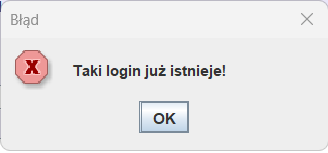
\includegraphics[width=0.4\textwidth]{figures/ThisLoginAlrExists.png}
\caption{Komunikat błędu - istniejący login}
\label{fig:loginExists}
\end{figure}

Przykładowy fragment kodu:
\begin{lstlisting}[style=javaStyle, caption={Walidacja unikalności loginu podczas rejestracji użytkownika}]
 public boolean loginExists(String login) {
        String sql = "SELECT 1 FROM users WHERE login = ?";
        try (Connection conn = DatabaseConnection.getConnection();
             PreparedStatement stmt = conn.prepareStatement(sql)) {
            stmt.setString(1, login);
            ResultSet rs = stmt.executeQuery();
            return rs.next();
        } catch (SQLException e) {
            e.printStackTrace();
        }
        return false;
    }    
/-----------------------------------------------------------------------\

 if (dao.loginExists(login)) {
            JOptionPane.showMessageDialog(null, "Taki login już istnieje!", "Błąd", JOptionPane.ERROR_MESSAGE);
            return;
        }

\end{lstlisting}

\subsection{Konflikt terminów wizyt}

Próba rezerwacji wizyty u lekarza w terminie, który koliduje z inną wizytą (z marginesem ±30 minut), powoduje wyświetlenie komunikatu o konflikcie (Rys. \ref{fig:visitConflict}).

\begin{figure}[H]
\centering
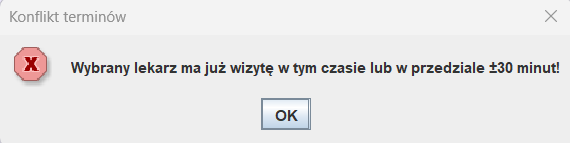
\includegraphics[width=0.6\textwidth]{figures/VisitKonflict.png}
\caption{Komunikat błędu - konflikt terminów wizyt}
\label{fig:visitConflict}
\end{figure}

Przykładowy fragment kodu:
\begin{lstlisting}[style=javaStyle, caption={Walidacja konfliktów wizyt ±30 minut u danego lekarza}]
public boolean hasDoctorConflict(int doctorId, LocalDateTime dateTime) {
    String sql = "SELECT COUNT(*) FROM visits WHERE doctor_id = ? AND ABS(EXTRACT(EPOCH FROM (visit_date - ?))) < 1800";

    try (Connection conn = DatabaseConnection.getConnection();
         PreparedStatement stmt = conn.prepareStatement(sql)) {

        stmt.setInt(1, doctorId);
        stmt.setTimestamp(2, Timestamp.valueOf(dateTime));

        ResultSet rs = stmt.executeQuery();
        if (rs.next()) {
            return rs.getInt(1) > 0;
        }
    } catch (SQLException e) {
        e.printStackTrace();
    }
    return false;
}

\end{lstlisting}

Powyższe przykłady stanowią tylko wybrane przypadki obsługi wyjątków w aplikacji. W projekcie zaimplementowano także inne wyjątki, takie jak błędy połączenia z bazą danych, walidacja danych wejściowych i inne komunikaty błędów użytkownika.



\chapter{Testowanie i podsumowanie}

\section{Testowanie systemu}

Testowanie aplikacji odbyło się na kilku poziomach: jednostkowym, integracyjnym oraz użytkowym.

\subsection{Testy jednostkowe}
Testy jednostkowe skupiały się na poprawnym działaniu poszczególnych metod klas modelu oraz DAO. Szczególną uwagę zwrócono na poprawność:

\begin{itemize}
\item walidacji danych wejściowych,
\item działania metod CRUD,
\item obsługi wyjątków bazodanowych i walidacyjnych.
\end{itemize}

Wszystkie testy jednostkowe zostały przeprowadzone ręcznie poprzez sprawdzanie poszczególnych funkcjonalności w środowisku IDE (IntelliJ IDEA).

\subsection{Testy integracyjne}
Testy integracyjne dotyczyły komunikacji między warstwą aplikacji (DAO) a bazą danych PostgreSQL. Testowano poprawność zapytań SQL oraz operacji CRUD realizowanych z poziomu aplikacji. Wszystkie operacje (dodawanie, edycja, usuwanie, filtrowanie) przebiegły pomyślnie, a wyniki testów potwierdziły poprawne funkcjonowanie aplikacji.

\subsection{Testy użytkowe}
Testy użytkowe zostały przeprowadzone z punktu widzenia końcowego użytkownika aplikacji. Testy obejmowały:

\begin{itemize}
\item logowanie i autoryzację użytkowników,
\item rezerwację wizyt z walidacją konfliktów terminów,
\item zarządzanie danymi pacjentów, lekarzy i wizyt przez sekretariat,
\item obsługę sytuacji wyjątkowych (np. błędny login lub zajęty termin wizyty).
\end{itemize}

Aplikacja wypadła pozytywnie, co potwierdziło intuicyjność oraz poprawność działania wszystkich zaimplementowanych funkcjonalności.

\section{Podsumowanie}

Głównym celem projektu było stworzenie funkcjonalnej aplikacji umożliwiającej zarządzanie wizytami lekarskimi. Projekt został zrealizowany zgodnie z wymaganiami, z wykorzystaniem technologii Java oraz Swing, z relacyjną bazą danych PostgreSQL. Zastosowano podejście obiektowe, które zapewniło czytelność oraz łatwość utrzymania kodu.

W przyszłości projekt może zostać rozbudowany o dodatkowe funkcjonalności, takie jak integracja z kalendarzem internetowym czy możliwość eksportu danych do popularnych formatów (np. CSV lub XLS).

Kod źródłowy projektu jest dostępny publicznie w repozytorium:
\begin{center}
\href{https://github.com/YevhenMarchak/Aplikacja_do_zarzadzania_wizytami_lekarskimi.git}{\texttt{github.com/YevhenMarchak/Aplikacja\_do\_zarzadzania\_wizytami\_lekarskimi}}
\end{center}

% --- < bibliografia > ---
\renewcommand{\emph}[1]{\textit{#1}}
\addcontentsline{toc}{section}{\textbf{Bibliografia}}

\nocite{*}
\bibliographystyle{plain}
\bibliography{bibliografia}
\renewcommand{\emph}[1]{\uline{#1}}

% --- < spisy > ---
\clearpage
\addcontentsline{toc}{section}{\textbf{Spis rysunków}}
\listoffigures
\clearpage

%\addcontentsline{toc}{section}{\textbf{Spis tabel}}
%\listoftables
%\clearpage

\addcontentsline{toc}{section}{\textbf{Spis listingów}}
\lstlistoflistings
\clearpage

% --- < aneksy > ---
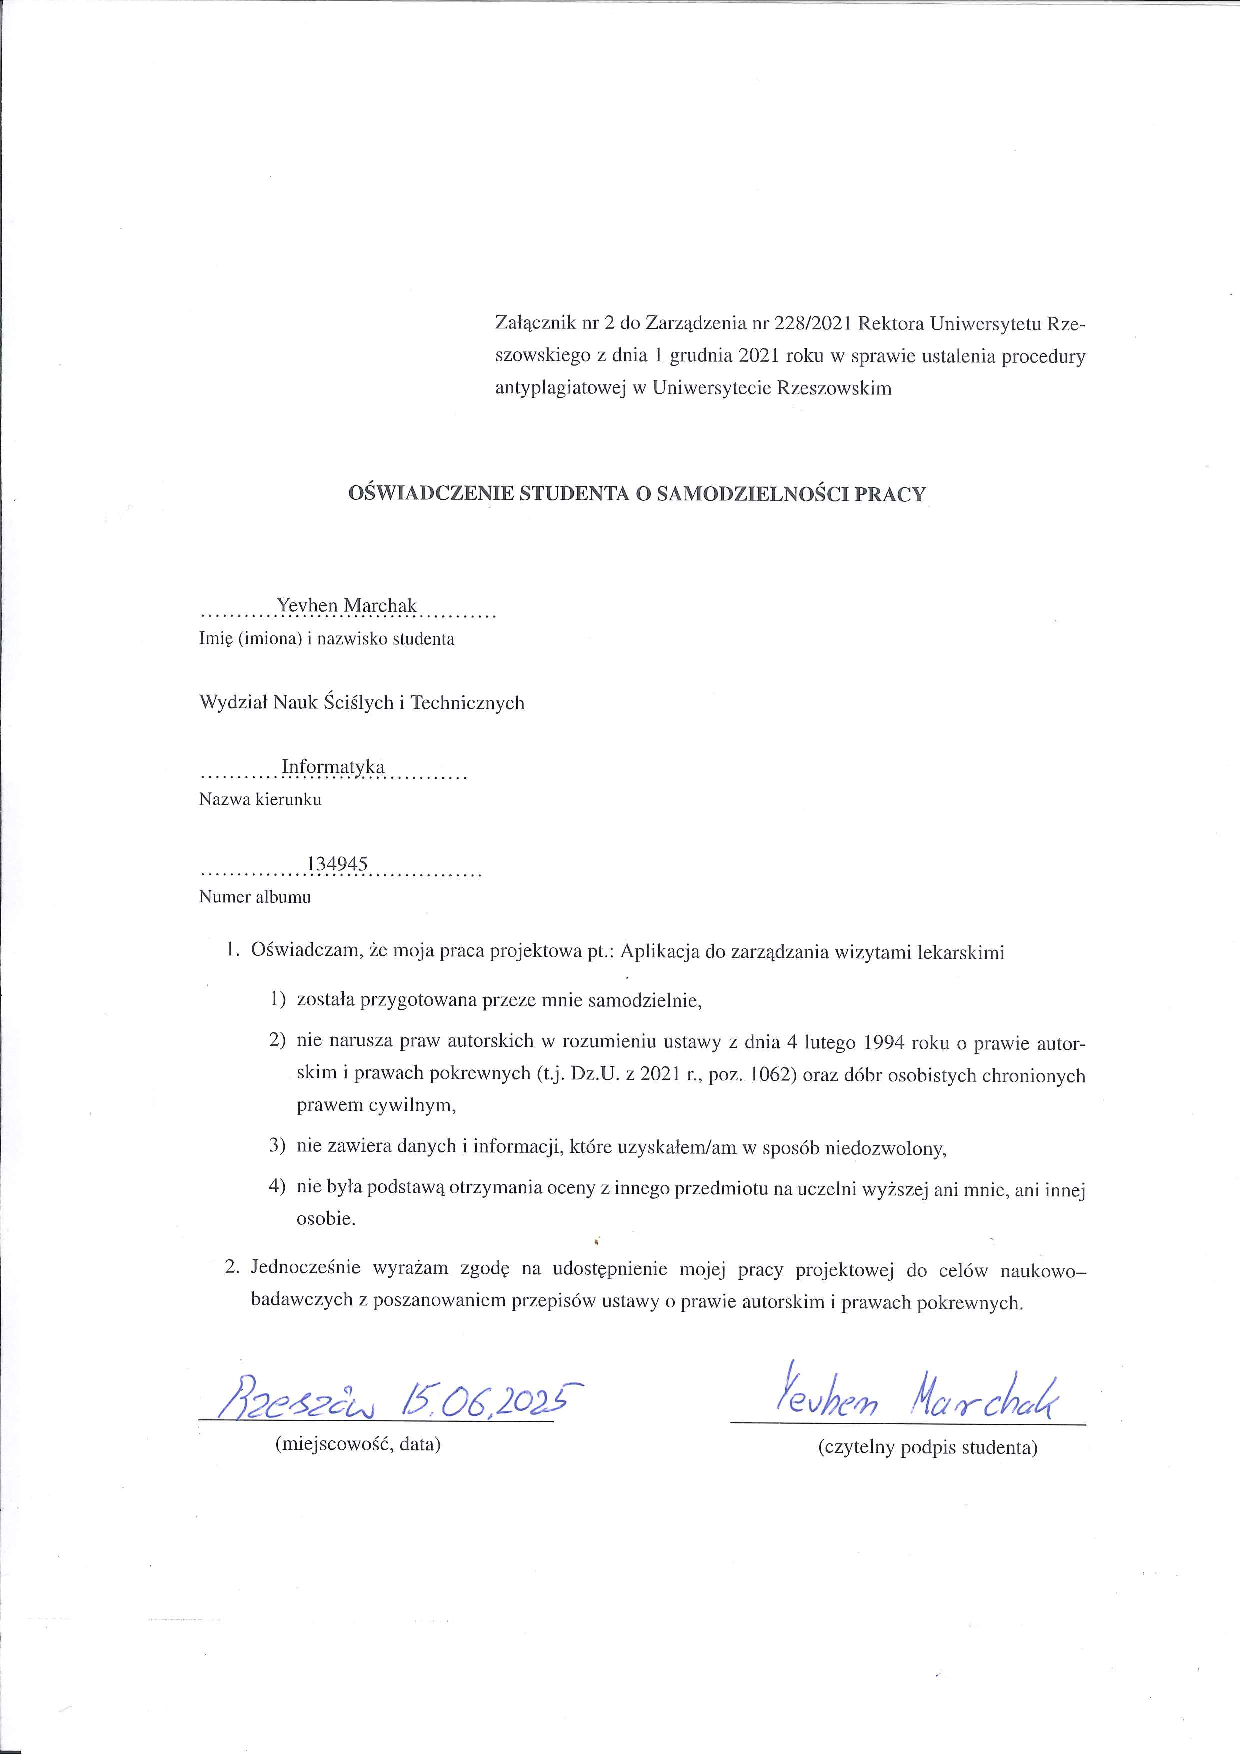
\includepdf[pages=-, width=\paperwidth, height=\paperheight]{figures/SkanZaswiadczenie.pdf}

\end{document}
